\documentclass{beamer}
\usepackage{pxfonts}
\usepackage{tikz}
\usepackage{ifthen}



\usetikzlibrary{calc,shadows}


\mode<presentation>
\usetheme[height=.75cm]{Rochester}

\title{GIT}
\author{Fr\'ed\'eric Vogels}
\institute[KHL]{KHLeuven}


\pgfkeys{
  /tikz/.cd,
  file/.style={fill=red!50,minimum width=.75cm,font=\tiny,draw},
  blob/.style={draw,fill=blue!50,font=\tiny,inner sep=.5mm},
  link/.style={-latex},
  note/.style={fill=gray!50,draw,drop shadow},
  note arrow/.style={->},
  caption/.style={fill=gray!50,draw,drop shadow,font={\Huge\sc}},
}

\newcommand{\bits}[1]{
  {
    \pgfmathparse{bin(128+mod(#1 * 229 + 73, 128))}\let\x\pgfmathresult
    \pgfmathparse{bin(128+mod(#1 * 541 + 111, 128)}\let\y\pgfmathresult
    \parbox{.9cm}{\centering\tt \x \\ \y}
  }
}


\begin{document}

\titlepage


\begin{frame}
  \frametitle{Without Version Control}
  \begin{center}
    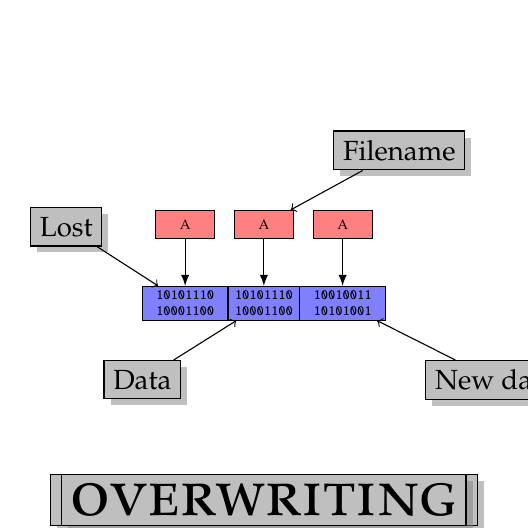
\begin{tikzpicture}
      \path[use as bounding box] (-3,-3) rectangle (3,3);
      \onslide<2-3>{
        \node[blob] (x) at (0,-.5) {\bits{1}};
        \node[file] (A) at ($ (x) + (0,1) $) {A};
        \draw[link] (A) -- (x);
        \node[caption] at (0, -3) {file creation};
      }
      \onslide<3>{
        \node[note,anchor=south west] (note A) at ($ (A.north east) + (.5,.5) $) {Filename};
        \draw[note arrow] (note A) -- (A);

        \node[note,anchor=north east] (note x) at ($ (x.south west) + (-.5,-.5) $) {Data};
        \draw[note arrow] (note x) -- (x);
      }

      \onslide<4-7>{
        \node[caption] at (0, -3) {overwriting};
      }
      \onslide<4-6>{
        \node[blob] (x) at (-1,-.5) {\bits{1}};
      }
      \onslide<4>{
        \node[file] (A) at ($ (x) + (0,1) $) {A};
        \draw[link] (A) -- (x);
      }
      \onslide<5-7>{
        \node[blob] (y) at ($ (x) + (2,0) $) {\bits{2}};
        \node[file] (A) at ($ (y) + (0,1) $) {A};
        \draw[link] (A) -- (y);
      }
      \onslide<6>{
        \node[note,anchor=south east] (note x) at ($ (x.north west) + (-.5,.5) $) {Lost};
        \draw[note arrow] (note x) -- (x);

        \node[note,anchor=north west] (note y) at ($ (y.south east) + (.5,-.5) $) {New data};
        \draw[note arrow] (note y) -- (y);
      }
    \end{tikzpicture}
  \end{center}
\end{frame}


\end{document}



%%% Local Variables: 
%%% mode: latex
%%% TeX-master: t
%%% End: 
